% COMS 6998, Fall 2026 -- P3: Evaluation Plan & Initial Results
% Uses the instructor-supplied, unmodified IEEEtran class.
\documentclass[conference,10pt,letterpaper]{IEEEtran}
\usepackage[T1]{fontenc}
\usepackage{cite}
\usepackage{graphicx}
\usepackage{booktabs}
\usepackage{tabularx}
\usepackage{flushend}
\usepackage[hyphens]{url}
\usepackage[hidelinks]{hyperref}

\title{B5: E-Graph-Augmented RTL Verification:\\
From Guard Acceleration to Proof Reuse}
\author{\IEEEauthorblockN{Chiyu Chen (cc5583), Mingyuan Zheng (mz3143), Yiwen Chen (yc4653)}
\IEEEauthorblockA{COMS 6998: AI-Native Computing $\mid$ Fall 2026\\
P3: Evaluation Plan \& Initial Results $\mid$ Due November 25, 2026, 11:59 PM ET}}

\begin{document}
\maketitle
\thispagestyle{plain}
\pagestyle{plain}

\section{Project Goal and Updates}
P2 asked whether E-graph feedback improves RTL coverage and token efficiency. Its controller retest tied at 11/12 fault types while the E-graph arm used 8.29\% more tokens; FIFO witness generation shortened SMT text but increased inclusive time. Our post-P2 review and guard optimizations show that ordinary rewriting and direct witness search recover most practical benefits. We therefore change the research question rather than search for favorable benchmarks.

\textbf{Updated question.} Can context-scoped, independently replayable E-graph explanations improve semantic maintenance of evolving LLM-generated RTL monitors over equally informed non-E-graph methods? The intended contribution is selective re-verification, reusable explanations and precise invalidation, not replacing SMT or assuming faster verification. Monitor correctness, proof coverage, cost and LLM utility are distinct endpoints. Prior work addresses E-graph hardware equivalence and conditional reasoning~\cite{wordlevel,colored}; we study their application to verification-property maintenance, not a new general equality-saturation algorithm.

\section{Evaluation Setup}
\textbf{Evidence pipeline.} We grade generated monitors against an independent specification. Python drives Yosys and Z3, with Icarus and Verilator for RTL replay. Given alarm predicates $P,Q$ under guard $G$, we check feasibility and both directions: $G\land P\land\neg Q$, then $G\land Q\land\neg P$. SAT/UNSAT distinguishes equality, weakening, strengthening and incomparability. Unknown and infeasible guards remain separate outcomes. Rust \texttt{egg} uses 23 checked Boolean rules and guard-certified typed facts. Certificates bind endpoints, types, guard, named steps and used dependencies; a separate checker replays them. Historical paths support reversal and composition through intermediate atoms. Re-certify only used equalities $a=b$ by checking $G\land(a\oplus b)$ is UNSAT in the new scope. After a disproven dependency, typed triage skips saturation only for confirmed non-equivalence; equivalent goals receive alternate proofs or SMT fallback. This is typed two-state snapshot reasoning, distinct from bounded model checking (BMC) of the DUT.

\textbf{Workloads.} Use original arbiter, Controller/SPI/I$^2$C guards, AXI FIFO and Frame Length Adjuster. The frozen corpus has 224 prior revision requests, six deduplicated assessments from real API histories, ten controlled ladder cases and 24 controlled aggregate requests (1/3/5/9 properties): 264 requests, 105 groups. Frame feedback holds out four of six internal mutants; the corpus is published, not a fresh hidden benchmark. M4 reserves a new 16-entry, 16-bit FIFO configuration and revisions of its stall monitors as an unevaluated holdout. Controlled edits are not natural LLM errors.

\textbf{Baselines and metrics.} Classical baselines are direct incremental SMT with equality paths/guard containment and ordinary reasoning with matched facts, solver cores and dependency reuse. Compare eager, cache-only, dependency-first and triage Egg under matched rules, types and budgets. Measure classifications, false equality acceptance, proof coverage, reuse, typed checks and inclusive time. Live Raw/Ordinary/Egg arms use matched tasks, common grading, actual tokens and rounds to qualification. An independent oracle grades after operational decisions.

\textbf{Platform.} Python 3.12, Z3 4.16, Rust 1.90/egg 0.11, Yosys and native simulators; live \texttt{gpt-6.1-sol}/low. Dependency experiments use Linux and MacBook (one primary/follow-up run each, plus a second Linux run). Mac hardware details are unrecorded; times are descriptive within host.

\section{Initial Results}
\textbf{Acceleration motivates the pivot.} Indexed matching preserves historical proofs, reducing Controller/SPI/I$^2$C medians 61.18/28.21/9.69 to 28.59/19.81/6.69 ms (12 paired repeats). Arbiter verification with nine certified rules falls from 135.91 to 11.49 ms (indexed Egg plus bit-parallel witnesses); direct bit-parallel search achieves the same coverage and defect results in 8.04 ms (six repeats/cell). Ordinary rewriting and Egg both reduce 148 Controller solver calls to 87; ordinary is faster.

\begin{figure*}[!t]
\centering
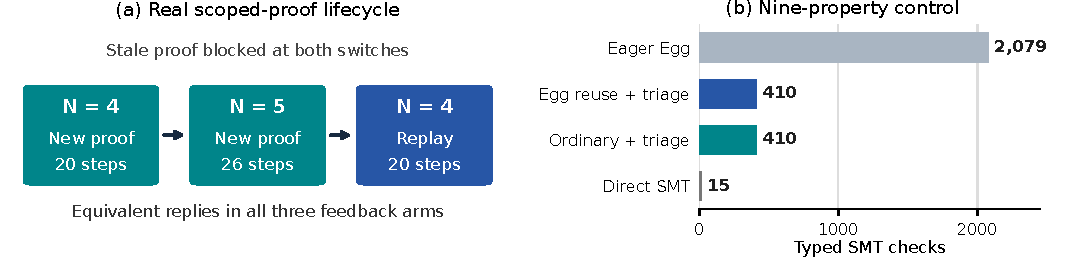
\includegraphics[width=\textwidth]{figure1.pdf}
\caption{(a) Real scoped-maintenance pilot ($N$ is tracked input length), three arms, three stages, nine responses: all replies qualify, but each stale carry is non-equivalent in the new scope. Egg records 20- and 26-step certificates and replays the first on return. (b) Offline controlled nine-property aggregate, six requests, one Mac run per arm, initial and failed-path checks included. Egg and ordinary triage tie; 399 of Egg's 410 checks are incurred at initial proof construction. Neither panel establishes a general RTL or LLM speedup.}
\label{fig:proof-reuse}
\end{figure*}

\textbf{Auditable evidence.} A checked arbiter waiver explains the unreachable branch; BMC and replay expose a reset-timing violation. The 70 Controller proofs use 50 distinct rules. Withdrawing each of 281 rules affects 71 proof/rule combinations: Egg and ordinary both recover 57; SMT proves the remaining 14. Both identify the same affected conclusions on ten controlled RTL edits.

\textbf{Actual RTL verification.} FIFO stall-hold assertion splitting preserves results: original 12-state BMC and induction pass; four field mutants fail and witnesses replay. Frame extends five local assertions to nine transaction obligations, increasing fixed mutant detection from 3/6 to 6/6. An independent handshake tracker supplies accepted history. Full-wrapper BMC passes eight safety properties at 18 states (single frame, length at most 12); six covers and two mutant counterexamples replay. Drain completion is finite-trace only, not unbounded correctness.

\textbf{Proof-carrying LLM.} Nine FIFO responses give identical correct monitors. Six Frame repairs end with identical monitors; missing associativity explains two Egg proof misses. Source-only DNF and ordinary reasoning both explain 220 archived alarms. On 24 offline fixture diagnostics, restricted-cube replaces DNF and raises checked proof coverage from 10/24 to 24/24. Our 18-response proof-carrying pilot sends 13 checked seed certificates, yet all 17 valid replies match. Three unaided transaction drafts already satisfy 9/9 properties; 18 later responses preserve them. Actual proof feedback works, but provides no observed quality gain.

\textbf{Context and reuse.} On 29 fixed pairs, scoped facts improve Egg proof coverage from 10/16 to 16/16 positives; ordinary matches 16/16 and all 13 negatives are rejected. A controlled TLAST monitor edit at $N=4$ creates 52 false and four missed alarms on main RTL traces. On the 224-request matrix (171 identities, 31 nonidentity equivalents, 22 negatives), all arms classify correctly. Shared graphs and prior paths reduce native builds 53 to 35, with eight prior-path requests. In the real nine-response $4\!\to\!5\!\to\!4$ pilot (Fig.~\ref{fig:proof-reuse}a), all arms qualify on first replies. Egg proofs enter subsequent prompts; Raw/Ordinary/Egg use 3,292/4,936/9,859 tokens. No reduction in model effort is observed.

\textbf{Dependency-driven results.} All six primary and four follow-up arms (two repeated) correctly classify 264 requests with zero false equalities. Egg retains proof paths for 59/61 nonidentity equivalents; ordinary covers 60/61. A controlled ladder uses $Q=P\land(N<8)$ and $R=P\land(N<9)$. Proofs at $N=4$ transfer $P\equiv R$ to $N=5$ by re-certifying two conditions. At $N=8$ the path is blocked but a new proof establishes equality. Triage skips two non-equivalent stale carries. Egg checks drop 581 to 516 on the matrix (ordinary 505, SMT 57); 181 to 153 on live (ordinary 153, SMT 10); 288 to 139 on the ladder. Across seven cohorts, checks drop 5,970 to 1,790 and builds 51 to 41; ordinary uses 1,779 and direct SMT 146. This mix is dominated by controlled aggregates.

Mac summed times fall 17.961 to 11.334 s, versus ordinary 2.724 s and SMT 2.546 s. Nine-property Egg triage beats direct once (0.811 vs.~0.972 s), but not ordinary (0.626 s). Matrix triage spends 7.032/7.911 s in 33 native invocations, including process/JSON. Mac/Linux proof stores, steps and queries agree; 12 groups per run differ only in node counts/IDs. Independent audits rebuild stores. Across 18,160 archived snapshots (30 traces), 31 new equivalent comparisons agree; main traces distinguish all eight negatives. Dependency experiments make no new API calls or temporal proofs. Protocols, scripts and raw evidence accompany the \href{https://github.com/Yiwen543/COMS6998-final-project}{project repository}.

\section{Planned Ablations and Next Steps}
For M4 (Dec.~7), prioritize \emph{demand-driven proof construction}: 399/410 nine-property checks precede the first proof. Search candidate derivations, certify only used obligations, replay certified steps and prune invalid paths; never accept speculative equality. Vary full vs.~on-demand discovery for Egg and equally informed ordinary/core methods; expect fewer cold checks without lost proof coverage. Compare shortest vs.~dependency-aware explanations, expecting fewer future invalidations; the $N=8$ blocked-but-equivalent case tests safe invalidation. Compare subprocesses with a persistent worker (fresh graph/request), expecting lower transport cost but unchanged proofs. M4 evaluates the frozen corpus and FIFO holdout against direct SMT and ordinary baselines, with median/IQR over five or more interleaved repeats/platform including startup and failures. Test concise proof dependencies vs.~matched ordinary LLM feedback on nontrivial revisions, retaining correct drafts. If baselines match, report the limit.

\begin{thebibliography}{2}
\bibitem{wordlevel} S. Coward, E. Morini, B. Tan, T. Drane, and G. Constantinides, ``Datapath Verification via Word-Level E-Graph Rewriting,'' FMCAD, 2023. \href{https://arxiv.org/abs/2308.00431}{arXiv:2308.00431}.
\bibitem{colored} E. Singher and S. Itzhaky, ``Colored E-Graph: Equality Reasoning with Conditions,'' 2023. \href{https://arxiv.org/abs/2305.19203}{arXiv:2305.19203}.
\end{thebibliography}
\end{document}
